\section{Experiments}
\label{sec:exp}

To measure Legion's ability to distribute work across a distributed machine, 
three benchmarks were developed and run on a small cluster under a variety
of configurations.  The cluster consists of four systems connected by a 40~Gb/s
Infiniband fabric.  Each system is powered by 2 Intel Xeon X5680 CPUs, each
with 6 cores, and 2 NVIDIA Tesla C2070 GPUs.  The systems were running Linux
with the standard OFED software stack, with GASnet using its ``ibv'' conduit
to run directly on top.

%%%%%%%%%%%%%%%%%%%%%%%%%%%%%%%%%%%%%%%%%%%%%%%%%%%%%%%%%%%%%%%%%%%%%%%%%

\subsection{Circuit Simulator}

The circuit simulator benchmark was designed to be representative of the
general class of finite-element simulations on irregular grids.  It relies
on many iterations using small stencils (e.g. just the neighboring nodes) to
propagate changes through the system, and each iteration requires communication
between neighboring nodes.  Careful partitioning of the system can minimize
the amount of information that must be exchanged, but the irregularity of the
underlying graph mandates similar irregularity in the sharing pattern.

The structure of the circuit simulator was presented in section~\ref{sec:ex}.
Our implementation uses CUDA to perform the computations on the GPU, and Legion
automatically handles the movement of data between the GPUs' memories and the
system memory, but only when necessary.  In fact, with the help of an
application-specific mapper, it is able to keep much of
the data permanently resident in a given GPU for the entirety of the simulation.
Figure~\ref{sfig:results1:perf} shows the relative speedup as the simulation is
spread over multiple nodes in the cluster.  The size of the circuit
being simulated is not changed as the node count increases.  This is therefore
a demonstration of ``strong scaling''.  Adding a second node to the simulation
speeds it up by 77\%, and with four nodes, the simulation is sped up by a total
of 216\% (i.e. a factor of 3.16x).

The bar graph in figure~\ref{sfig:results1:timers} breaks down the simulation's
run time by where it was spent.  The times are summed over all threads, so 
perfect linear scaling would keep the bars flat in this graph.  The total
overhead introduced by Legion is XX \% for the single-node case.
shows a breakdown of the
total amount of time spent 

\pgfplotsset{every axis legend/.append style={
  font=\tiny,
  at={(0.02,0.98)},
  anchor=north west}}


\begin{figure}
  \centering
  \subfigure[Performance Scaling]{
    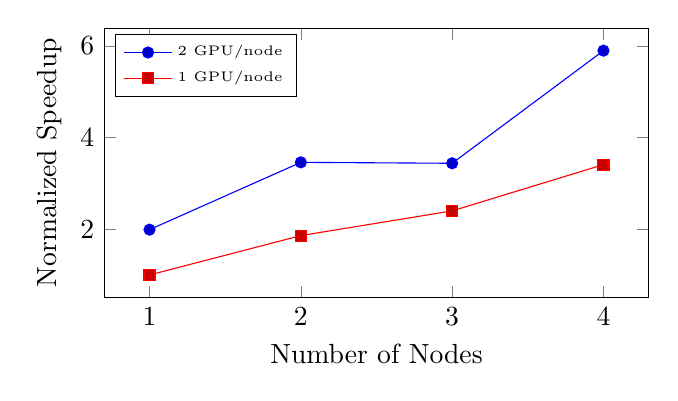
\begin{tikzpicture}
      \begin{axis}[xlabel=Number of Nodes,ylabel=Normalized Speedup,height=5cm,width=8.5cm,xtick={1,2,3,4}]
        \addplot coordinates {
% num gpus = 2
  (1, 1.99)
  (2, 3.46)
  (3, 3.44)
  (4, 5.90)
        };
        \addplot coordinates {
% num gpus = 1
  (1, 1.00)
  (2, 1.86)
  (3, 2.40)
  (4, 3.41)
        };
      \legend{2 GPU/node,1 GPU/node}
      \end{axis}
    \end{tikzpicture}
    \label{sfig:results1:perf}
  }

  \subtable[Execution Time Breakdown]{
   \tiny
    \begin{tabular}{c@{\hspace{2pt}}cD{.}{.}{3}D{.}{.}{3}@{\hspace{2pt}}D{.}{.}{3}@{\hspace{2pt}}D{.}{.}{3}@{\hspace{2pt}}D{.}{.}{3}@{\hspace{2pt}}D{.}{.}{3}@{\hspace{2pt}}D{.}{.}{3}}
\toprule
GPUs/ & \# \\
node & nodes & \multicolumn{1}{c}{Wall Clock} & \multicolumn{1}{c}{Application} & \multicolumn{1}{c}{Copies} & \multicolumn{1}{c}{High-level} & \multicolumn{1}{c}{Low-level} & \multicolumn{1}{c}{Mapper} & \multicolumn{1}{c}{System} \\
\midrule
\multirow{4}{*}{$1$} & $1$ & 106.892 & 105.387 & 1.578 & 0.003 & 21.624 & 0 & 0\\
 & $2$ & 57.388 & 105.407 & 10.348 & 0.003 & 15.177 & 0 & 0.001\\
 & $3$ & 44.552 & 105.41 & 11.935 & 0.003 & 11.695 & 0 & 0.002\\
 & $4$ & 31.368 & 105.42 & 12.875 & 0.004 & 8.419 & 0 & 0.003\\
\midrule
\multirow{4}{*}{$2$} & $1$ & 53.787 & 105.397 & 1.857 & 0.004 & 10.953 & 0 & 0\\
 & $2$ & 30.923 & 105.415 & 10.716 & 0.004 & 7.937 & 0 & 0.002\\
 & $3$ & 31.037 & 105.414 & 12.558 & 0.004 & 7.996 & 0 & 0.001\\
 & $4$ & 18.103 & 105.42 & 13.747 & 0.004 & 4.638 & 0 & 0.003\\
\bottomrule \\
    \end{tabular}
    \label{sfig:results1:timers}
  }
  \caption{Circuit Simulator Results}
\end{figure}

\pgfplotsset{every axis legend/.append style={
  font=\tiny,
  at={(0.02,0.98)},
  anchor=north west}}

%%%%%%%%%%%%%%%%%%%%%%%%%%%%%%%%%%%%%%%%%%%%%%%%%%%%%%%%%%%%%%%%%%%%%%%%%

\subsection{Fluid}

To show that Legion remains efficient for regular partitioning cases as well,
we have implemented a particle simulation benchmark, based heavily on the
{\tt fluidanimate} benchmark from the PARSEC suite.  The simulation uses a
cyclic 2D grid of cells instead of PARSEC's 3D grid with boundaries, and 
The fluid benchmark used here differs slightly from the PARSEC version.  It
uses a 2D grid of cells instead of a 3D grid, but the computations being 
performed are preserved.
Although the 
simulation is moving and colliding individual particles, those particles
are placed in cells that make up a regular grid, and the time steps and grid
sizes are chosen carefully to ensure that a particle can only interact with
particles in the same cell or in one immediately adjacent.  The grid is
divided into blocks to be processed by individual threads, with only the
particles in the edge cells being of interest to other threads.  The PARSEC
implementation uses fine-grained locking and the assumption of cache
coherence to access neighboring particles, but neither of these are available
across a cluster.  Our fluid benchmark replaces these accesses with rings of
explicit edge, or \emph{ghost}, cells that are exchanged between adjacent
blocks several times in each iteration.  The capturing of these inter-block
interactions through edge cells and the partitioning of those cells into
subregions shoulds the runtime the ability to schedule data movement in
advance and do a more precise enforcement of ordering constraints (e.g.
requiring a task to wait only for the tasks in the previous pass that computed
one of the ghose cells this task needs).

Figure~\ref{sfig:results2:perf} shows the performance of the fluid benchmark
relative to the serial Legion version.  MORE TEXT HERE.

The bar chart in figure~\ref{sfig:results2:timers} shows MORE STUFF.

\begin{figure}
  \centering
  \subfigure[Performance Scaling]{
    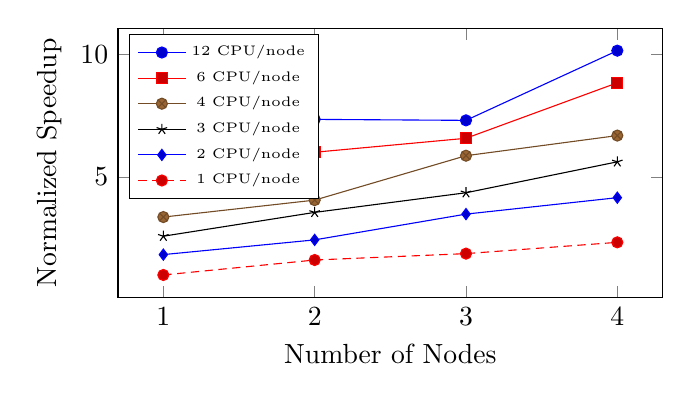
\begin{tikzpicture}
      \begin{axis}[xlabel=Number of Nodes,ylabel=Normalized Speedup,height=5cm,width=8.5cm,xtick={1,2,3,4}]
        \addplot coordinates {
% 12 CPUs
  (1, 5.29)
  (2, 7.34)
  (3, 7.30)
  (4, 10.14)
        };
        \addplot coordinates {
% 6 CPUs
  (1, 4.51)
  (2, 6.00)
  (3, 6.57)
  (4, 8.83)
        };
        \addplot coordinates {
% 4 CPUs
  (1, 3.36)
  (2, 4.05)
  (3, 5.86)
  (4, 6.68)
        };
        \addplot coordinates {
% 3 CPUs
  (1, 2.58)
  (2, 3.55)
  (3, 4.35)
  (4, 5.61)
        };
        \addplot coordinates {
% 2 CPUs
  (1, 1.83)
  (2, 2.43)
  (3, 3.48)
  (4, 4.15)
        };
        \addplot coordinates {
% 1 CPUs
  (1, 1.00)
  (2, 1.61)
  (3, 1.87)
  (4, 2.33)
        };
      \legend{12 CPU/node,6 CPU/node,4 CPU/node,3 CPU/node,2 CPU/node,1 CPU/node}
      \end{axis}
    \end{tikzpicture}
    \label{sfig:results2:perf}
  }

  \subtable[Execution Time Breakdown]{
   \tiny
    \begin{tabular}{c@{\hspace{2pt}}cD{.}{.}{3}D{.}{.}{3}@{\hspace{2pt}}D{.}{.}{3}@{\hspace{2pt}}D{.}{.}{3}@{\hspace{2pt}}D{.}{.}{3}@{\hspace{2pt}}D{.}{.}{3}@{\hspace{2pt}}D{.}{.}{3}}
\toprule
GPUs/ & \# \\
node & nodes & \multicolumn{1}{c}{Wall Clock} & \multicolumn{1}{c}{Application} & \multicolumn{1}{c}{Copies} & \multicolumn{1}{c}{High-level} & \multicolumn{1}{c}{Low-level} & \multicolumn{1}{c}{Mapper} & \multicolumn{1}{c}{System} \\
\midrule
\multirow{4}{*}{$1$} & $1$ & 40.718 & 38.486 & 0.008 & 0.996 & 0.544 & 0 & 0\\
 & $2$ & 25.365 & 43.602 & 0.455 & 2.027 & 0.682 & 0 & 0.043\\
 & $3$ & 21.808 & 49.256 & 0.513 & 2.377 & 0.765 & 0 & 0.06\\
 & $4$ & 17.476 & 53.181 & 0.501 & 2.912 & 0.743 & 0 & 0.072\\
\midrule
\multirow{4}{*}{$2$} & $1$ & 22.289 & 38.55 & 0.009 & 1.694 & 0.68 & 0 & 0\\
 & $2$ & 16.787 & 51.081 & 0.573 & 2.373 & 0.756 & 0 & 0.056\\
 & $3$ & 11.706 & 49.502 & 0.733 & 2.661 & 0.749 & 0 & 0.072\\
 & $4$ & 9.817 & 50.798 & 0.86 & 2.755 & 0.735 & 0 & 0.1\\
\midrule
\multirow{4}{*}{$3$} & $1$ & 15.799 & 38.507 & 0.01 & 2.056 & 0.765 & 0 & 0\\
 & $2$ & 11.462 & 48.698 & 0.951 & 2.682 & 0.819 & 0 & 0.109\\
 & $3$ & 9.363 & 50.786 & 1.282 & 2.976 & 0.767 & 0 & 0.081\\
 & $4$ & 7.26 & 51.778 & 1.285 & 3.172 & 0.818 & 0 & 0.117\\
\midrule
\multirow{4}{*}{$4$} & $1$ & 12.11 & 39.296 & 0.011 & 2.17 & 0.827 & 0 & 0\\
 & $2$ & 10.05 & 49.799 & 1.145 & 3.023 & 0.82 & 0 & 0.24\\
 & $3$ & 6.951 & 51.216 & 1.367 & 3.137 & 0.798 & 0 & 0.12\\
 & $4$ & 6.093 & 52.183 & 1.216 & 3.317 & 0.782 & 0 & 0.135\\
\midrule
\multirow{4}{*}{$6$} & $1$ & 9.031 & 40.265 & 0.013 & 2.536 & 0.969 & 0 & 0\\
 & $2$ & 6.79 & 48.992 & 0.946 & 3.182 & 0.937 & 0 & 0.145\\
 & $3$ & 6.199 & 51.904 & 1.061 & 3.752 & 0.909 & 0 & 0.185\\
 & $4$ & 4.612 & 52.603 & 1.238 & 3.712 & 0.872 & 0 & 0.222\\
\midrule
\multirow{4}{*}{$12$} & $1$ & 7.704 & 45.959 & 0.03 & 4.01 & 1.765 & 0 & 0\\
 & $2$ & 5.547 & 65.432 & 1.019 & 4.762 & 1.328 & 0 & 0.232\\
 & $3$ & 5.577 & 68.74 & 1.059 & 5.922 & 1.384 & 0 & 0.322\\
 & $4$ & 4.017 & 67.662 & 1.19 & 4.882 & 1.22 & 0 & 1.485\\
\bottomrule \\
    \end{tabular}
    \label{sfig:results2:timers}
  }

  \caption{Fluid Results}
\end{figure}

%%%%%%%%%%%%%%%%%%%%%%%%%%%%%%%%%%%%%%%%%%%%%%%%%%%%%%%%%%%%%%%%%%%%%%%%%

\subsection{Tree Search}

The circuit simulation was able to count on a good static, if irregular,
partition of its workload, but that is not possible in some cases.  One
such example arises in ray tracing, in which the components of a scene to be
rendered are partitioned in a binary tree to minimize the number of expensive
object intersection tests that must be performed.  By traversing its path 
through the tree, a ray is able to efficiently skip entire chunks of the 
scene that it is guaranteed not to intersect with.  The trees tend to be
highly imbalanced (often intentionally so), and the set of rays that traverse
the tree tend to have similar path.  Both of these factors contribute to
large fluctuations in the load on any particular part of the tree, complicating
attempts to statically partition the tree.  The {\tt Tree Search} benchmark
explores Legion's ability to load-balance tasks in a locality-aware manner.

The benchmark constructs an irregular binary tree, and then partitions it into
roughly subregions that have roughly equal numbers of nodes.  Partition
crossings are annotated on the tree and traversal tasks are re-spawned when
a ray crosses into another partition.  Load imbalances will occur, but when
they do, the default mapper's ability to provide a set of tasks with good
locality should minimize the amount of data that must be copied around.  To
measure this benefit, each run is also done with the tree partitioning 
disabled.  This denies the mapper the locality information it would need to 
make good choices, reducing it to making essentially random choices.

Figure~\ref{sfig:results3:perf} shows performance of the tree search test
relative to the single node with partitioning case. MORE TEXT HERE.

\begin{figure}
  \centering
  \subfigure[Performance Scaling]{
    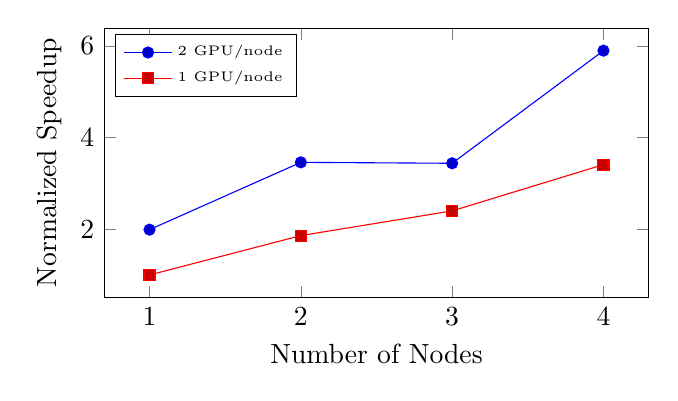
\begin{tikzpicture}
      \begin{axis}[xlabel=Number of Nodes,ylabel=Normalized Speedup,height=5cm,width=8.5cm,xtick={1,2,3,4}]
        \addplot coordinates {
% num gpus = 2
  (1, 1.99)
  (2, 3.46)
  (3, 3.44)
  (4, 5.90)
        };
        \addplot coordinates {
% num gpus = 1
  (1, 1.00)
  (2, 1.86)
  (3, 2.40)
  (4, 3.41)
        };
      \legend{2 GPU/node,1 GPU/node}
      \end{axis}
    \end{tikzpicture}
    \label{sfig:results3:perf}
  }

  \subtable[Execution Time Breakdown]{
   \tiny
    \begin{tabular}{c@{\hspace{2pt}}cD{.}{.}{3}D{.}{.}{3}@{\hspace{2pt}}D{.}{.}{3}@{\hspace{2pt}}D{.}{.}{3}@{\hspace{2pt}}D{.}{.}{3}@{\hspace{2pt}}D{.}{.}{3}@{\hspace{2pt}}D{.}{.}{3}}
\toprule
GPUs/ & \# \\
node & nodes & \multicolumn{1}{c}{Wall Clock} & \multicolumn{1}{c}{Application} & \multicolumn{1}{c}{Copies} & \multicolumn{1}{c}{High-level} & \multicolumn{1}{c}{Low-level} & \multicolumn{1}{c}{Mapper} & \multicolumn{1}{c}{System} \\
\midrule
\multirow{4}{*}{$1$} & $1$ & 106.892 & 105.387 & 1.578 & 0.003 & 21.624 & 0 & 0\\
 & $2$ & 57.388 & 105.407 & 10.348 & 0.003 & 15.177 & 0 & 0.001\\
 & $3$ & 44.552 & 105.41 & 11.935 & 0.003 & 11.695 & 0 & 0.002\\
 & $4$ & 31.368 & 105.42 & 12.875 & 0.004 & 8.419 & 0 & 0.003\\
\midrule
\multirow{4}{*}{$2$} & $1$ & 53.787 & 105.397 & 1.857 & 0.004 & 10.953 & 0 & 0\\
 & $2$ & 30.923 & 105.415 & 10.716 & 0.004 & 7.937 & 0 & 0.002\\
 & $3$ & 31.037 & 105.414 & 12.558 & 0.004 & 7.996 & 0 & 0.001\\
 & $4$ & 18.103 & 105.42 & 13.747 & 0.004 & 4.638 & 0 & 0.003\\
\bottomrule \\
    \end{tabular}
    \label{sfig:results3:timers}
  }
  \caption{Tree Search Results}
\end{figure}

